\documentclass[border=10pt]{standalone}
\usepackage[svgnames]{xcolor}
\usepackage{amsmath}
\usepackage{pgfplots}
\pgfplotsset{compat=newest}
\usepackage[sfdefault]{FiraSans}
\usepackage{FiraMono}
\renewcommand*\familydefault{\sfdefault}
\begin{document}
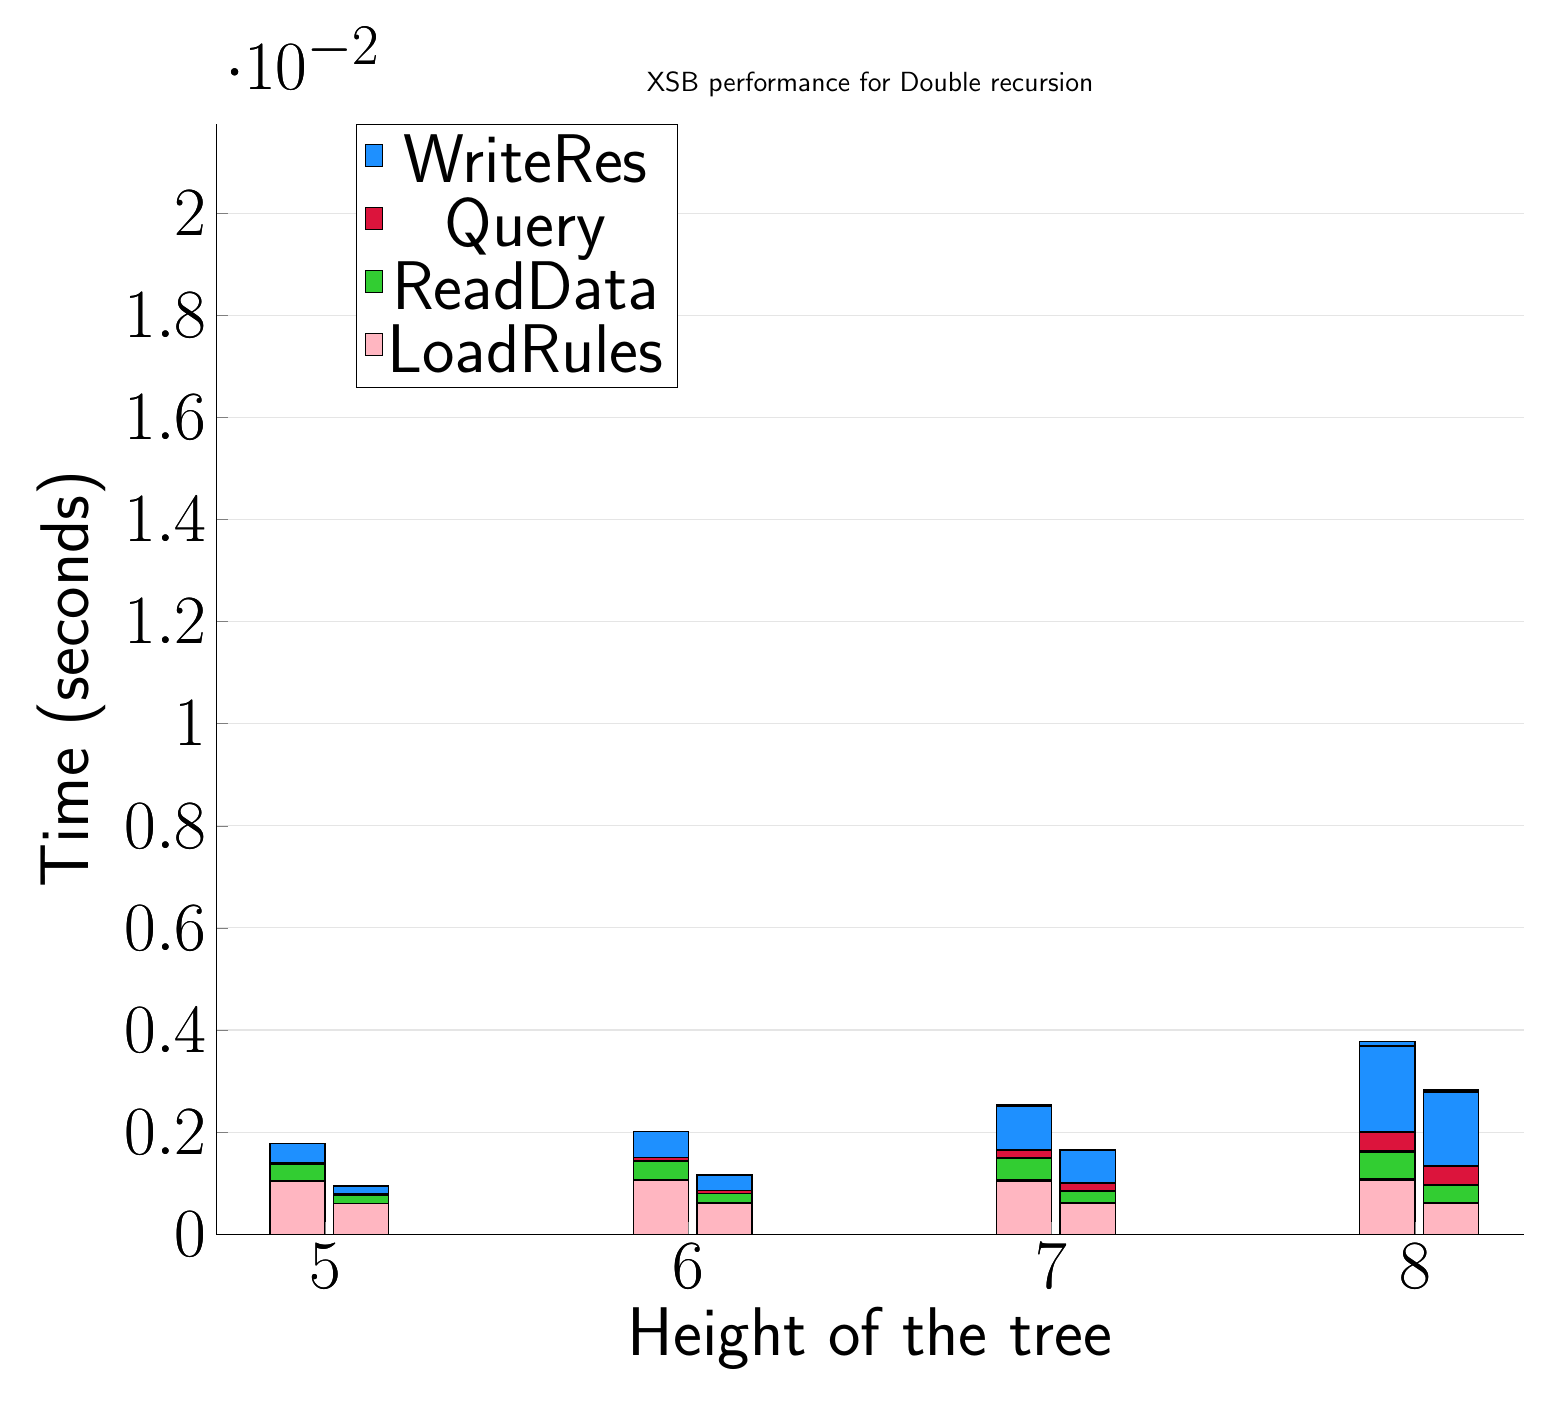
\begin{tikzpicture}
\begin{axis}[
   ybar stacked,
   title={XSB performance for Double recursion},
   bar shift=-10pt,
   width=1.5\textwidth,
   bar width=0.7cm,
   ymajorgrids, tick align=inside,
   major grid style={draw=gray!20},
   xtick=data,
   ymin=0, ymax=0.02175771713256836,
   axis x line*=bottom,
   axis y line*=left,
   enlarge x limits=0.1,
   legend style={
       at={(0.23, 1)},
       anchor=north,
       legend columns=1,
       font=\Huge,
   },
   ylabel={Time (seconds)},
   xlabel={Height of the tree},
   label style={font=\Huge},
   tick label style={font=\Huge},
]
\addlegendimage{fill=DodgerBlue, draw=black, line width=0.2pt}
\addlegendentry{WriteRes}
\addlegendimage{fill=Crimson, draw=black, line width=0.2pt}
\addlegendentry{Query}
\addlegendimage{fill=LimeGreen, draw=black, line width=0.2pt}
\addlegendentry{ReadData}
\addlegendimage{fill=LightPink, draw=black, line width=0.2pt}
\addlegendentry{LoadRules}
\addplot +[fill=LightPink, draw=black, line width=0.5pt] coordinates {
    (5, 0.0010392189025878909)
    (6, 0.0010601758956909168)
    (7, 0.001044058799743653)
    (7, 0.001056694984436035)
    (7, 0.001061654090881347)
    (8, 0.001049327850341798)
    (8, 0.0010823011398315417)
    (8, 0.001065540313720703)
};
\addplot +[fill=LimeGreen, draw=black, line width=0.5pt] coordinates {
    (5, 0.0003370523452758789)
    (6, 0.00037202835083007815)
    (7, 0.00043978691101074217)
    (7, 0.0004363298416137697)
    (7, 0.0004344701766967775)
    (8, 0.000564408302307129)
    (8, 0.0005377769470214842)
    (8, 0.0005626201629638672)
};
\addplot +[fill=Crimson, draw=black, line width=0.5pt] coordinates {
    (5, 3.421306610107418e-05)
    (6, 6.842613220214844e-05)
    (7, 0.0001568078994750978)
    (7, 0.0001576900482177734)
    (7, 0.0001537084579467773)
    (8, 0.0003885746002197267)
    (8, 0.00038833618164062515)
    (8, 0.00038518905639648435)
};
\addplot +[fill=DodgerBlue, draw=black, line width=0.5pt] coordinates {
    (5, 0.00036628246307373057)
    (6, 0.0005138635635375976)
    (7, 0.0008689880371093754)
    (7, 0.0008561849594116207)
    (7, 0.0008855104446411127)
    (8, 0.0016829490661621105)
    (8, 0.0016907691955566416)
    (8, 0.0017577171325683586)
};
\end{axis}
\begin{axis}[
   ybar stacked,
   bar shift=13pt,
   width=1.5\textwidth,
   bar width=0.7cm,
   ymajorgrids, tick align=inside,
   major grid style={draw=none},
   xtick=data,
   ymin=0, ymax=0.02175771713256836,
   axis x line*=none,
   axis y line*=none,
   enlarge x limits=0.1,
   label style={font=\Huge},
   tick label style={font=\Huge},
]
\addplot +[fill=LightPink, draw=black, line width=0.5pt] coordinates {
    (5, 0.0006029000000000001)
    (6, 0.0006119999999999998)
    (7, 0.0006027999999999999)
    (7, 0.0006178999999999999)
    (7, 0.0006127000000000001)
    (8, 0.0006044000000000004)
    (8, 0.0006211000000000003)
    (8, 0.0006079999999999998)
};
\addplot +[fill=LimeGreen, draw=black, line width=0.5pt] coordinates {
    (5, 0.0001550999999999999)
    (6, 0.00018570000000000018)
    (7, 0.00024310000000000022)
    (7, 0.00024140000000000007)
    (7, 0.00024150000000000018)
    (8, 0.0003522999999999995)
    (8, 0.0003447999999999998)
    (8, 0.0003491000000000001)
};
\addplot +[fill=Crimson, draw=black, line width=0.5pt] coordinates {
    (5, 3.009999999999974e-05)
    (6, 6.329999999999964e-05)
    (7, 0.00015109999999999988)
    (7, 0.00014750000000000022)
    (7, 0.0001474999999999999)
    (8, 0.0003725000000000001)
    (8, 0.00036830000000000055)
    (8, 0.0003709999999999997)
};
\addplot +[fill=DodgerBlue, draw=black, line width=0.5pt] coordinates {
    (5, 0.00015820000000000027)
    (6, 0.00030090000000000027)
    (7, 0.0006467000000000006)
    (7, 0.0006446999999999996)
    (7, 0.0006536999999999999)
    (8, 0.0014425)
    (8, 0.0014566999999999996)
    (8, 0.0014952000000000001)
};
\end{axis}
\end{tikzpicture}

\end{document}
